\chapter{Att bygga ett system i ROS}
\chapterprecis{\LARGE{---- Martin Lundberg ----}}
\label{cha:indiv-report-lundberg}

\section{Inledning}
\label{sec:introduction-lundberg}

I ROS finns det många verktyg för att bygga upp ett system. ROS gör det enkelt att köra fler processer och kommunicera mellan dessa. Det hjälper även till att tydliggöra uppdelningar av ett program i separata moduler som enkelt kan återanvändas och vidareutvecklas separat utan att påverka de övriga modulerna.


\subsection{Syfte}
\label{sec:purpose-lundberg}

Syftet med den här rapporten är att utforska olika metoder i ROS för att bygga upp ett system. Rapporten ska även jämföra lösningarna i ROS med andra metoder för att ge fler perspektiv på hur ett system kan byggas upp. 

\subsection{Frågeställning}
\label{sec:issue-lundberg}

Följande frågeställningar ska behandlas och besvaras i denna rapport.

\begin{enumerate}
	\item Hur kan en arkitektur implementeras i ROS?
	
	\item Hur påverkade valet att använda ROS uppbyggnaden av systemet?
	
	\begin{comment}
		\item Vilka erfarenheter kan man få av att ta fram och implementera en arkitektur?
	\end{comment}
\end{enumerate}


\section{Bakgrund}
\label{sec:background-lundberg}

ROS från vårt perspektiv, varför vi använde ROS, sammanhanget för rapporten

I det projekt som utvecklats och beskrivits i huvuddelen av denna rapport användes ROS redan från ett tidigt skede. En anledning till att just ROS valdes var för att projektets kund hade det som önskemål, dock såg projektmedlemmarna tidigt att ROS förde med sig många fördelar. Användningen av ROS planerades redan i arkitekturen som är utformad helt med förutsättningen att ROS skulle användas för implementationen.

I denna rapport utreds hur ROS kan användas i implementationen av en arkitektur. Arkitekturen hade som mål att vara så modulär som möjligt då det skulle underlätta för projektets kund som vill kunna vidareutveckla olika delar av systemet i framtiden.

I ett sent skede i projektet behövde stora ändringar göras i arkitekturen vilket gjorde att ROS uteslöts helt. Detta gav ytterligare ett perspektiv att utgå från i utredningen.


\section{Teori}
\label{sec:theory-lundberg}

\subsection{ROS}
ROS står för Robot Operating System men är inte ett fullt operativsystem i den traditionella meningen. Istället är det ett system som körs i ett vanligt operativsystem och som ger användaren möjlighet att på ett enkelt sätt köra flera processer och kommunicera mellan dessa \cite{quigley2009ros}. En process som körs i ROS kallas för en nod och ROS tillhandahåller verktyg för att styra dessa noder. Det är ofta en bra tumregel att tänka att en nod motsvarar en modul i arkitekturen.

ROS har även verktyg för att på ett enkelt och strukturerat sätt kommunicera mellan noder genom meddelanden (eng. messages). Dessa meddelanden kan skickas på två olika sätt:

\begin{enumerate}
	\item Genom att en nod publicerar på en namngiven kanal (eng. topic) som en annan nod kan lyssna på.
	
	\item En nod kan tillhandahålla en service som en annan nod kan kalla på för att utföra något arbete och få tillbaka resultatet i form av ett meddelande.
\end{enumerate}

Den här rapporten ska utforska hur dessa verktyg kan användas för att bygga upp ett system.

\subsection{Pipe and filter-modellen}
En välkänd modell för att bygga upp mjukvarusystem är pipe and filter-modellen. Den beskrivs av Garlan och Shaw \cite{garlan1993introduction} som en modell där varje komponent i systemet har bestämda indata och utdata. Komponenterna behandlar indatan och producerar utdata som kan skickas vidare till nästa steg i modellen.

I en traditionell pipe and filter-modell behandlas indatan kontinuerligt så att utdata produceras innan hela strömmen av indata har nått fram, därav namnet filter. I detta projekt användes dock ett specialfall av modellen där varje komponent kräver ett helt block av indata som sedan behandlas för att producera ett block av utdata. Det ska noteras att trots att varje modul endast tar kompletta block av indata snarare än strömmar så kan modulerna internt arbeta med strömmar av data och inkrementellt ta fram resultatet.


\section{Metod}
\label{sec:method-lundberg}

\subsection{Arkitekturens framtagande}
Arkitekturen för systemet har tagits fram med en iterativ process. Det första steget var att tänka igenom olika use cases för systemet och utifrån det ta fram de funktioner som programvaran måste innehålla. Detta inledande arbete resulterade i en systemanatomi som användes i det kommande arbetet.

Ett viktigt mål med arkitekturen var att systemet skulle vara modulärt. Tidigt i arbetet togs det fram en pipe and filter-modell där resultatet från ett steg skickas vidare som indata till nästa steg. En stor fördel med denna modell är att den gör det möjligt att byta ut enskilda delar utan att göra om hela systemet. \cite{garlan1993introduction}. Detta är något som uppfyller de krav på moduläritet och underhållbarhet som ställdes på systemet.

Nästa steg var att se vilka funktioner som var relaterade till varandra och bestämma vilka noder systemet skulle bestå av och även hur dessa skulle kommunicera med varandra. Det var tydligt att programmets funktionalitet kunde delas upp i tre distinkta delar:

\begin{enumerate}
	\item punktmolnshantering
	
	\item meshgenerering
	
	\item hantering av 3D-skrivare.
\end{enumerate}

Utöver de delarna behövdes även ett sätt att styra processen. För detta ändamål infördes ett grafiskt användargränssnitt och även ett kommandoradsgränssnitt som skulle kunna initiera hela eller delar av processen.

Då projektet byggde vidare på ett system kallat TreeD från förra året för att styra hårdvaran behövde även det tidigare systemet tas i åtanke när arkitekturen togs fram. Fler alternativ för att kommunicera med det tidigare systemet utforskades men i slutändan beslutades det att en egen nod skulle kalla på det tidigare systemets kommandoradsgränssnitt för att på så vis slippa sätta sig in i tidigare kod för att lista ut vilka funktioner som behövde kallas.

\subsection{Användandet av ROS}

För att bygga systemet i ROS togs ett första förslag på en arkitektur fram där de moduler som beskrevs ovan motsvarade en varsin ROS-nod. För att kommunicera med varandra skulle noderna använda sig av topics för att ta emot kommandon och skicka resultatet av utförda beräkningar. Att använda topics hade fördelen att det är ett enkelt och snabbt sätt att komma igång. Det var dock ett naivt sätt att implementera systemet i det här fallet då en topic-baserad lösning gör väldigt lite för att upprätthålla den tänkta arkitekturen. Eftersom vilken nod som helst kan lyssna på en topic blir det svårare att se kommunikationsvägarna mellan olika noder och därför blir det även svårare för en utomstående att förstå systemets uppbyggnad och vidareutveckla systemet.

För att göra systemet tydligare togs en ny arkitektur fram som istället var baserad på service-anrop. I denna arkitektur tillhandahåller modulerna en service som en annan nod kan kalla på för att utföra ett specifikt arbete. När arbetet är utfört returneras resultatet till noden som utförde service-anropet. Detta system gör det mycket tydligare vad de olika noderna gör och hur de kommunicerar med varandra och det är den slutgiltiga arkitekturen i ROS som togs fram för projektet.


\subsection{Dokumentering av processen}
Under framtagandet av arkitekturen dokumenterades arbetet kontinuerligt i form av mötesprotokoll och diverse skisser och blockscheman som togs fram. Stora delar av arbetet med arkitekturen finns dokumenterat i projektets arkitekturbeskrivning (KÄLLA?) där alla beslut som tagits om arkitekturen finns. Den innehåller även motiveringar till de beslut som fattats och, i relevanta fall, alternativa lösningar som diskuterades men som inte kom med i den slutgiltiga arkitekturen.


\section{Resultat}
\label{sec:results-lundberg}

Sent i projektet stötte gruppen på problem som inte gick att lösa inom en rimlig tidsram. Därför behövde projektets mål omdefinieras och på grund av det togs även ny arkitektur fram, denna gång utan ROS. I detta avsnitt visas båda de arkitekturer som togs fram för projektet. 

\subsection{Arkitekturen i ROS}
Den ROS-baserade arkitektur som togs fram för projektet visas i figur \ref{fig:arkitektur}. Varje block i figuren motsvarar en nod i ROS och kommunikationsvägarna mellan noderna illustreras med pilar. All kommunikation mellan noderna utförs i form av service-anrop i ROS.

\begin{figure}[h]
	\centering
	\includegraphics[width=15cm]{figures/arkitektur.png}
	\caption{Systemets arkitektur i ROS.}
	\label{fig:arkitektur}
\end{figure}

\subsection{Arkitekturen utan ROS}

Den nya arkitekturen som togs fram utan ROS är uppbyggd enligt samma modell i grunden. Dock är den skriven helt i C++ och uppbyggd med hjälp av klasser som tillhandahåller den funktionalitet som tidigare låg i noder. Den nya arkitekturen använder inte heller det tidigare projektet TreeD så wrappern för den mjukvaran är borttagen. I detta system läses punktmolnsfiler in av klienten som sedan använder funktionaliteten i klasserna för att behandla punktmolnen. Klassindelningen och kopplingen mellan dem beskrivs i figur \ref{fig:klasser}.

\begin{figure}[h]
	\centering
	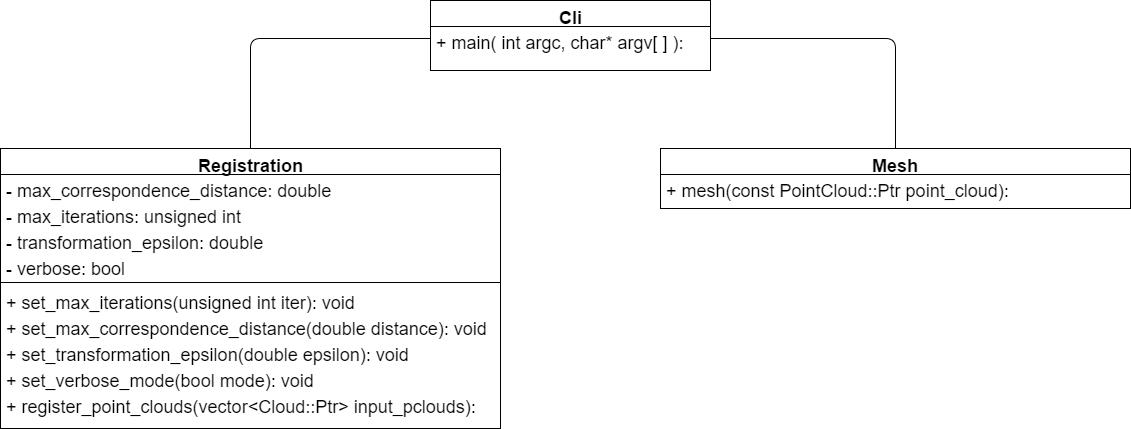
\includegraphics[width=15cm]{figures/klassdiagram.png}
	\caption{Systemets arkitektur utan ROS.}
	\label{fig:klasser}
\end{figure}


\section{Diskussion}
\label{sec:discussion-lundberg}

Resultatet av arbetet var två olika arkitekturer och implementationer av i grunden samma arkitekturidé. Detta ger möjlighet att jämföra ett system byggt i ROS med i princip samma system byggt utan ROS.

Under arbetet med att ta fram och implementera dessa arkitekturer framkom en del för- och nackdelar med båda alternativen. Dessa diskuteras i detta avsnitt.

\begin{comment}
– 6.1 Resultat
• Fanns alternativa implementationssätt?
• Vad återstår för att kunden skall få ut fullt värde av
produkten?
• Lyckades ni förbättra/fortsätt något från tidigare projekt?
• Viktigaste lärdomar inför framtiden.
– 6.2 Metod
• Vilka konsekvenser fick de valda metoderna för resultaten?
• Fanns det alternativ?
• Källkritik
– 6.3 Arbetet i ett vidare sammanhang
• Samhälleliga aspekter
• Miljöaspekter
• Etiska aspekter

Stelt system med services, kan inte se delresultat

Skriva om hur det var att gå från ROS till klasser med metoder

"Den utvecklade arkitekturen jämförs med en alternativ hypotetisk arkitektur, vilken uppvisade lägre komplexitet och större portabilitet. Den är dock inte lika lättanvänd tillsammans med andra ROS-system."

Diskutera kring att vi endast använde services och att det därför var enkelt att översätta till klasser jämfört med topics.
\end{comment}

\section{Slutsatser}
\label{sec:conclusions-lundberg}

\begin{comment}
- Återkoppling till frågeställningar
– Nåddes syftet?
– Viktigaste lärdomar

En viktig insikt under arbetet var att en prestigelös dialog mellan gruppmedlemmarna är väldigt viktigt för att få ut det bästa resultatet.
\end{comment}

%%%%%%%%%%%%%%%%%%%%%%%%%%%%%%%%%%%%%%%%%%%%%%%%%%%%%%%%%%%%%%%%%%%%%%
%%% person-report.tex ends here
